%%%%%%%%%%%%%%%%%%%%%%%%%%%%%%%%%%%%%%%%%%%%%%%%
\begin{frame}
		\frametitle{}
		\Background[1] 
	    \begin{center}
		{ {\Huge 第三章~~薛定谔方程 (I)\\(6学时)}}
	    \end{center}    
\end{frame}
%%%%%%%%%%%%%%%%%%%%%%%%%%%%%%%%%%%%%%%%%%%%%

\section{1.薛定谔方程基础}
\subsection{薛定谔方程}
\begin{frame}
	\frametitle{}  
	\begin{block}	{量子力学有关波函数的基本结论}
	\begin{itemize}
		\item 	波函数$\Psi$完全描述体系的状态,
		\item 	波函数的模方与粒子出现的概率成比例,$\omega \sim |\Psi|^2$
		\item 	波函数的演化服从薛定谔方程 : $\hat{E} \Psi = \hat{H}  \Psi $ 
	\end{itemize}
	薛定谔方程是量子力学基本方程,与牛顿力学的牛顿第二定理地位相当
	\end{block}	
\end{frame}

%%%%%%%%%%%%%%%%%%%%%%%%%%%%%%%%%%%%%%%%%%%%%
\begin{frame}
	\frametitle{方程的建立}
	\begin{alertblock} {可能思路}  
		\begin{itemize}
			\Item 	\textbf{1:}  最小作用量原理 $\int\limits_{t_1}^{t_2} \delta L d t =0 $\\ 
			\Item 	\textbf{2:}  波粒二象性\\ 
			~\\ 
			\Item 	\textbf{3:}  基本假设,不能从现有理论推导\\
            ~\\ 
            \begin{quote}
            "It is not possible to derive it from anything you know. It came out of the \alert{\faHeartbeat} of Schr$\ddot{o}$dinger"\\
            \rightline{$\cdots$ R. P. Feynman \hspace{3em}}   
            \end{quote}
		\end{itemize}
	\end{alertblock}
\end{frame}
\begin{frame}
	\frametitle{含时薛定谔方程}
	标准形式:    
	 \begin{equation*}
		i\hbar \frac{\partial }{\partial t} \Psi (\overrightarrow{r},t ) =\left [ -\frac{\hbar^2}{2\mu }\nabla ^2 + V(\overrightarrow{r},t ) \right ]\Psi (\overrightarrow{r}, t ) 
	\end{equation*}
	若取 $ \displaystyle  i\hbar \frac{\partial }{\partial t} ~~\to ~~ \hat{E} ~~, ~~  -\frac{\hbar^2}{2\mu }\nabla ^2 + V(\vec{r},t ) ~~\to ~~ \hat{H} $ \\
	算符形式:   \\ 
	\begin{equation*}
		\hat{E} ~ \Psi (\overrightarrow{r},t )  = \hat{H} ~ \Psi (\overrightarrow{r},t )  
	\end{equation*}
\end{frame}

\subsection{分离变量}

\begin{frame}
	\frametitle{分离变量}
	\begin{alertblock} {薛定谔方程$\hat{E} \Psi = \hat{H}  \Psi $ 为什么难求解?因为很难分离变量!}
		~~\\
		多粒子体系的波函数:
		\begin{equation*}
			\Psi (\vec{r_1},\vec{r_2},...,\vec{r_n},t )
		\end{equation*}		
		多粒子体系的哈密顿量:
		\begin{equation*}
			\hat{H} ~=\sum_{i=1}^{n} -\frac{\hbar^2}{2\mu }\nabla ^2 _i + \sum_{i=1}^{n} V(\vec{r_i},t) + \sum_{i,j=1, i\ne j}^{n}  U(\vec{r_i},\vec{r_j}) 
		\end{equation*}	
		有可能分离变量吗?条件呢?
	\end{alertblock}	
\end{frame}

\begin{frame}
\frametitle{分离变量(1)->固有值问题->定态薛定谔方程}
	若势函数$V(\vec{r},t ) $不显含时间$t$,时间变量可分离 \\ \vspace{0.3cm}
	方程: { $ \displaystyle i \hbar \frac{\partial }{\partial t} \Psi (\vec{r},t ) =\left [- \frac{\hbar^2}{2\mu }\nabla ^2 + V(\vec{r}) \right ]\Psi (\vec{r},t ) $}  \\  \vspace{0.3cm}
	\alert{解:}  设  $\Psi (\vec{r},t )  = \Psi (\vec{r} ) f(t) $ , 代回方程 \\ \vspace{0.6em}
	{ $ \displaystyle i\hbar \Psi (\vec{r})  \frac{\partial }{\partial t} f(t)=f(t) \left [ -\frac{\hbar^2}{2\mu }\nabla ^2 + V(\vec{r}) \right ]\Psi (\vec{r}) $}  \\ 	
	{ $ \displaystyle i\hbar \frac{1}{f(t)}  \frac{\partial }{\partial t} f(t)= \frac{1}{\Psi (\vec{r}) } \left [ -\frac{\hbar^2}{2\mu }\nabla ^2 + V(\vec{r}) \right ]\Psi (\vec{r}) =E $}  \\ 	
\end{frame}

\begin{frame}
	\frametitle{}
	得两个微分方程:\\  \vspace{0.3cm}
	I、演化问题(方程)  \[ \displaystyle  i\hbar \frac{1}{f(t)}  \frac{\partial }{\partial t} f(t)=E \]   
	解方程,得:$\displaystyle  f(t) =e^{-iEt/\hbar}$ \\  \vspace{0.6cm}
	II、固有值问题(定态薛定谔方程) \[\displaystyle   \left [ -\frac{\hbar^2}{2\mu }\nabla ^2 + V(\vec{r}) \right ]\Psi (\vec{r}) =E \Psi (\vec{r})  \]   
	算符形式:\[   \hat{H} \Psi (\vec{r}) =E \Psi (\vec{r})    \] 
	哈密顿量决定固有值问题(定态薛定谔方程)求解难度!	
\end{frame}

\begin{frame}
	\frametitle{分离变量(2)->单粒子定态薛定谔方程}
	多粒子体系的定态薛定谔方程:   
	\begin{equation*}
		\left [ \sum\limits_{i=1}^{n} \hat{H}_i + \sum_{i,j=1, i\ne j}^{n}  U(\vec{r_i},\vec{r_j}) \right ]	\Psi (\vec{r_1},\vec{r_2},...,\vec{r_n})=E 	\Psi (\vec{r_1},\vec{r_2},...,\vec{r_n})
	\end{equation*}		
	\alert{解:}  	对于无相互作用体系, 
	有$ U(\vec{r_i},\vec{r_j}) =0 $,\\
	 $ \hat{H}= \sum\limits_{i=1}^{n} (-\dfrac{\hbar^2}{2\mu }\nabla ^2 _i + V(\vec{r_i})) =\sum\limits_{i=1}^{n} \hat{H}_i \qquad (1)$\\   \vspace{0.3cm}
	方程可进一步分离变量!令 : \\
	 $\displaystyle \begin{cases}
	   	\Psi (\vec{r_1},\vec{r_2},...,\vec{r_n}) = \Psi (\vec{r_1}) \Psi (\vec{r_2})...\Psi (\vec{r_n}) \qquad (2) \\
		E= E_1+ E_2 + ... + E_n=\sum\limits_{i=1}^{n} \hat{E}_i \qquad (3)
	\end{cases}$ \\ \vspace{0.3em}
 	把(1)(2)(3)代回原方程
\end{frame}

\begin{frame}
	\frametitle{}
	获得如下方程
	\[ \sum\limits_{i=1}^{n} \hat{H}_i\Psi (\vec{r_1}) \Psi (\vec{r_2})...\Psi (\vec{r_n})= \sum\limits_{i=1}^{n} \hat{E}_i\Psi (\vec{r_1}) \Psi (\vec{r_2})...\Psi (\vec{r_n}) \]
	进一步简化,得单粒子定态薛定谔方程组\\
	$\displaystyle \begin{cases}
		\hat{H}_1\Psi (\vec{r_1})=E_1 \Psi (\vec{r_1})  \\  
		\hat{H}_2\Psi (\vec{r_2})=E_2 \Psi (\vec{r_2})  \\
		\dots\\
		\hat{H}_n\Psi (\vec{r_n})=E_n \Psi (\vec{r_n})  \\
	\end{cases}$ \\	
\end{frame}

\begin{frame}
	\frametitle{分离变量(3)->一维定态薛定谔方程} 
	单粒子定态薛定谔方程标准型
	\begin{equation*}
		\left [ -\dfrac{\hbar^2}{2\mu }\nabla ^2 + V(x,y,z) \right ]\Psi (x,y,z) =E \Psi (x,y,z)  
	\end{equation*}		
	\alert{解:} 若势函数 $ V(x,y,z)=V_1(x)+V_2(y)+V_3(z) $,则  $ \hat{H}=\hat{H}(x)+\hat{H}(y)+\hat{H}(z) $\\
	进一步分离变量:设  $$\Psi (x,y,z)  = \Psi_1 (x)\Psi_2 (y) \Psi_3 (z), \qquad  E= E_x+ E_y+E_z $$ \\
	代回, 得一维薛定谔方程(组)
	$\displaystyle \begin{cases}
		\hat{H}(x)\Psi_1 (x)=E_x \Psi_1 (x) \\
		\hat{H}(y)\Psi _2 (y)=E_y \Psi _2 (y)  \\
		\hat{H}(z)\Psi _3 (z)=E_z \Psi _3 (z) 
	\end{cases}$ \\	
\end{frame}

\begin{frame}
	\frametitle{}	
	如果势函数 $$ V(x,y,z)=V(r,\theta,\varphi) =V_1(r)+V_2(\theta)+V_3(\varphi) $$
	令  $$ \hat{H}=\hat{H}(r)+\hat{H}(\theta)+\hat{H}(\varphi) $$
	分离变量得一维薛定谔方程:\\
	$\displaystyle \begin{cases}
		\hat{H}(r)\Psi_1 (r)=E_r \Psi_1 (r) \\
		\hat{H}(\theta)\Psi _2 (\theta)=E_\theta \Psi _2 (\theta)  \\
		\hat{H}(\varphi)\Psi _3 (\varphi)=E_\varphi \Psi _3 (\varphi) 
	\end{cases}$ \\	
\end{frame}

%%%%%%%%%%%%%%%%%%%%%%%%%%%%%%%%%%%%%%%%%%%%%
\section{2.无限深势阱}

\begin{frame}
	\frametitle{}
	\begin{exampleblock} {例1、	一维无限深势阱I}
	一粒子处于如下一维无限深势阱,求解含时薛定谔方程\\
 	{ $ \displaystyle 
	V(x)=\left \{ 
	\begin{array}{cccc}
		0	~~ ~~ 0<x<a \\  
		+\infty ~~x<0, x>a\\
	\end{array}
	\right.
	$} \\
	\end{exampleblock} %2
	\alert{解:} 	势函数不显含时间t,含时薛定谔方程可分离变量,时间演化方程已求得(见前),现求定态薛定谔方程:\\
	{  $ \displaystyle 
	\left \{ 
	\begin{array}{cccc}
		\left [ -\dfrac{\hbar^2}{2\mu} \dfrac{\mathrm{d} ^2}{\mathrm{d} x^2} +0 \right ]\Psi(x)=E\Psi(x)  ~~ ~~ 0<x<a,~~~~~~~~ (1)  \\ 
		\\	
		\left [ -\dfrac{\hbar^2}{2\mu} \dfrac{\mathrm{d} ^2}{\mathrm{d} x^2} +\infty \right ]\Psi(x)=E\Psi(x)  ~~ ~~ x<0,~ x>a ~~~~~(2)  \\
	\end{array}
	\right.
	$} \\
\end{frame}

\begin{frame}
	\frametitle{}
	方程(2):解为  $\Psi(x) = 0$ \\ 
    方程(1):令 $ k^2= \dfrac{2\mu E}{\hbar ^2} $, 方程是如下边值问题:  \\ 
	{ $ \displaystyle 
		\begin{cases}
			\Psi''(x) + k^2	\Psi(x)=0  \\
			\Psi(0)=0~,~~ \Psi(a)=0 ~~~~~
		\end{cases}
		$} \\  \vspace{0.3cm}
    特征方程有两虚根,通解为:\\
     	\begin{equation*}
  			\Psi(x) = A\cos(kx) +B\sin(kx) 
    	\end{equation*}
    取$x=0, x=a$,  代入上式,由零边值条件得:\\
   	\hspace{2cm} $A=0, ~~~~ \sin ka =0$  \\  \vspace{0.3cm}
	有:$ka=n\pi  \to  k=\dfrac{n\pi}{a} = \sqrt{\dfrac{2\mu E}{\hbar ^2}}$    \\ 
\end{frame}

\begin{frame}
	\frametitle{}
	固有值(能级):{ $E_n = \dfrac{n^2\pi^2\hbar^2}{2\mu a^2} (n=1,2,3,...)$} \\
	能级间隔:  $\triangle E = E_{n+1}-E_n=\dfrac{\pi^2 \hbar^2}{2\mu a^2} (2n+1)$ \\ 
	固有函数: $ \Psi_n(x) = B_n\sin(\dfrac{n\pi}{a}x)  = \sqrt{\dfrac{2}{a}} \sin(\dfrac{n\pi}{a}x)$ \\ 
	\alert{归一化}: $ \int \limits_{0}^{a}  \Psi_n ^*(x)  \Psi_n(x)dx = \int \limits_{0}^{a}  |B_n| ^2 \sin^2(\dfrac{n\pi}{a}x) dx =1$  \\ 
	系数:$B_n=\sqrt{\dfrac{2}{a}}$ \\ 
	解函数: \\
	{  $ \displaystyle 
		\Psi_n(x,t)= \left \{ 
		\begin{array}{cccc}
			\sqrt{\dfrac{2}{a}} \sin(\dfrac{n\pi}{a}x) e^{-\dfrac{i}{\hbar} E_n t} ~~~~   0<x<a \\
			0 ~~~~~~~~~~~~~~~~~~~~~~~ x<0,x>a  
		\end{array}
		\right.
		$} \\	
\end{frame}

\begin{frame}
	\frametitle{}
  叠加解:
	  \[\Psi_(x,t)= A_n \psi_n(x,t)\]

  (1)给出定解条件,如何求$A_n$ \\ 
  (2)势阱有变化.如何解方程\\ \vspace*{0.6em}
	 {$ \displaystyle 
   V(x)=\left \{ 
   \begin{array}{cccc}
	   0+1	~~ ~~ 0<x<a \\  
	   +\infty ~~x<0, x>a\\
   \end{array}
   \right.
   ;$} \\ \vspace*{0.3em}
   {$ \displaystyle  V(x)=\left \{ 
	  \begin{array}{cccc}
		  0	~~ ~~ -a<x<a \\  
		  +\infty ~~x<-a, x>a\\
	  \end{array}
	  \right.
  ;$}\\ \vspace*{0.3em}
  {$ \displaystyle   V(x)=\left \{ 
	  \begin{array}{cccc}
		  0	~~ ~~ -\frac{a}{2}<x<\frac{a}{2} \\  
		  +\infty ~~x<-\frac{a}{2}, x>\frac{a}{2}\\
	  \end{array}
	  \right.
   $} \\
\end{frame}

\begin{frame}
	\frametitle{}
	%\usetikzlibrary {datavisualization.formats.functions} 
	\begin{center}
	\begin{tikzpicture}[baseline, scale=.6]
	\datavisualization [ scientific axes, 
		visualize as smooth line/.list={sin,cos,tan}, style sheet=strong colors,
		style sheet=vary dashing,
		sin={label in legend={text=$\Psi_1$}}, 
		cos={label in legend={text=$\Psi_2 $}}, 
		tan={label in legend={text=$\Psi_3 $}}, 
		data/format=function ]
		data [set=sin] {
			var x : interval [0:1];
			func y = sin(pi* \value x r ) * 1.414;
		}
		data [set=cos] {
			var x : interval [0:1];
			func y = sin(2*pi* \value x r ) * 1.414;
		}
		data [set=tan] {
			var x : interval [0:1];
			func y = sin(3*pi* \value x r ) * 1.414;
		};
	\end{tikzpicture} \\ \vspace{0.3cm}
	\end{center}
	\begin{center}
	\begin{tikzpicture}[baseline, scale=.6]
		\datavisualization [ scientific axes, 
		visualize as smooth line/.list={sin,cos,tan}, style sheet=strong colors,
		style sheet=vary dashing,
		sin={label in legend={text=$|\Psi_1|^2$}}, 
		cos={label in legend={text=$|\Psi_2|^2$}}, 
		tan={label in legend={text=$|\Psi_3|^2$}}, 
		data/format=function ]
		data [set=sin] {
			var x : interval [0:1];
			func y = sin(pi* \value x r ) *sin(pi* \value x r ) *2;
		}
		data [set=cos] {
			var x : interval [0:1];
			func y = sin(2*pi* \value x r ) *sin(2*pi* \value x r ) *2;
		}
		data [set=tan] {
			var x : interval [0:1];
			func y = sin(3*pi* \value x r ) * sin(3*pi* \value x r ) *2;
		};
	\end{tikzpicture}
	\end{center}
\end{frame}

\begin{frame}
	\frametitle{}
	\begin{exampleblock} {例2、无限深势阱II}
		设有一粒子处于如下一维无限深势阱中,求解薛定谔方程\\
		{ $ \displaystyle 
			V(x)=\left \{ 
			\begin{array}{cccc}
				0	~~ ~~ |x|<\dfrac{a}{2} \\  
				+\infty ~~|x|>\dfrac{a}{2}\\
			\end{array}
			\right.
		$} \\
	\end{exampleblock}
	\alert{解:} 	势函数与上例存在平移关系, 令$x' =x+a/2$\\
	有:  $  \sin(\dfrac{n\pi}{a}x') =\sin(\dfrac{n\pi}{a} (x+a/2)) $ \\
	\hspace{2cm}$=\sin \dfrac{n\pi}{a} x \cos \dfrac{n\pi}{2} + \cos \dfrac{n\pi}{a} x \sin \dfrac{n\pi}{2}  $ \\ 
	n为偶数: $E_{2m} = \dfrac{2m^2\pi^2\hbar^2}{\mu a^2} $\\
	\hspace{2cm}$ \Psi_{2m}(x)= B_{2m} \sin(\dfrac{2m\pi}{a}x) $,   \\
\end{frame}

\begin{frame}
	\frametitle{}
	n为奇数:  $E_{2m+1} = \frac{(2m+1)^2\pi^2\hbar^2}{2\mu a^2} $ \\
	\hspace{2cm}$ \Psi_{2m+1}(x)= B_{2m+1} \cos(\dfrac{(2m+1)\pi}{a}x) $,  \\
	归一化,求系数 ... \\	 \vspace{0.6cm}	
	\textbf{如果把势阱宽改为2a}, 直接求解, 可得: \\
	固有值(能级):{ $E_n = \dfrac{n^2\pi^2\hbar^2}{8\mu a^2} (n=1,2,3,...)$} \\
	固有函数: $ \Psi_n(x)= \sqrt{\dfrac{2}{a}} \sin(\dfrac{n\pi}{a}(x+a)) $ \\  \vspace{0.6cm}	
	比较两种解之间的关系!	明确势阱平移与伸缩后解的写法。
\end{frame}

\begin{frame}
	\frametitle{}
	\begin{exampleblock} {例3、无限深势阱III}
	求解一维无限深势阱的非定常问题 \\
		{ $ \displaystyle 
			\begin{cases}
				i\hbar \dfrac{\partial }{\partial t} \Psi = -\dfrac{\hbar^2}{2\mu } \dfrac{\partial ^2 \Psi }{\partial ^2  x ^2 } , ~~ (0<x<L, t>0) \\
				\Psi (0,t) =0, ~~ \Psi (L,t) =0 \\
				\Psi (x,0) =f(x)  \\
			\end{cases}
		$} \\
	\end{exampleblock}
	\alert{解:} 	令$\Psi (x,t) =\Psi (x) T(t) $ ,  代回方程, 得:\\
	{ $ \displaystyle 
	\begin{cases}
		\Psi''(x) + k^2	\Psi(x)=0  \\
		\Psi(0)=0~,~~ \Psi(L)=0 ~~~~~
	\end{cases}
	$} \\
	固有值: $E_n = \dfrac{n^2\pi^2\hbar^2}{2\mu L^2} (n=1,2,3,...)$\\
	固有函数: $ \Psi_n(x) = \sin(\dfrac{n\pi}{L}x) $ 	 \\ 
\end{frame}

\begin{frame}
	\frametitle{}
	时间函数: $T_n(t)  = \exp(-i E_n t /\hbar) $ \\
	级数解为:  $ \Psi(x,t)  = \sum\limits_{n=1}^{\infty}  B_n \exp(-i E_n t /\hbar)  \sin(\dfrac{n\pi}{L}x)  $ \\
	取 t=0, 代入初值条件, 得:  $ f(x)= \sum\limits_{n=1}^{\infty}  B_n \sin(\dfrac{n\pi}{L}x)  $ \\
	得系数:  $ B_n= \dfrac{2}{L} \int\limits_{0} ^{L}  \sin(\dfrac{n\pi}{L}x) dx, ~~ (n=1,2,3,...) $ \\
\end{frame}

\begin{frame}
	\frametitle{作业}
	1、求定态薛定谔方程\\ 
	$\begin{array}{lllllllll}
		& \begin{cases}
			\Psi'' (x) +\dfrac{2\mu E}{\hbar ^2} \Psi(x) =0,~~ |x|<a/2 \\
			\Psi(-a/2) =\Psi(a/2) =0\\
		\end{cases}\\	
	\end{array}$ \\ 
	2、求解非定常问题\\
	$\begin{array}{lllllllll}
		& \begin{cases}
			i\hbar \dfrac{\partial }{\partial t} \Psi = -\dfrac{\hbar^2}{2\mu } \dfrac{\partial ^2 \Psi }{\partial ^2  x ^2 } , ~~ (0<x<L, t>0) \\
			\Psi (0,t) =0, ~~ \Psi (L,t) =0 \\
			\Psi (x,0) =f(x)  \\
		\end{cases}\\
	\end{array}$ \\ 
	3、求三维无限势阱问题\\
	$ ~~~~	V(x,y,z)=\left \{ 
	\begin{array}{cccc}
		0	~~ ,~~ 0<x,y,z<a \\  
		+\infty ,~~others\
	\end{array}
	\right. $ 	
	4. 求自由粒子的一维薛定谔方程\\
\end{frame}

%%%%%%%%%%%%%%%%%%%%%%%%%%%%%%%%%%%%%%%%%%%%%
\section{3.量子谐振子与厄密方程}

\subsection{相互作用势}

\begin{frame}
	\frametitle{相互作用势}
	\begin{exampleblock} {例1、相互作用势的二阶近似}
		半经验Lennard-Jones势(如图所示)\\ \vspace{0.6em }
	   \centerline{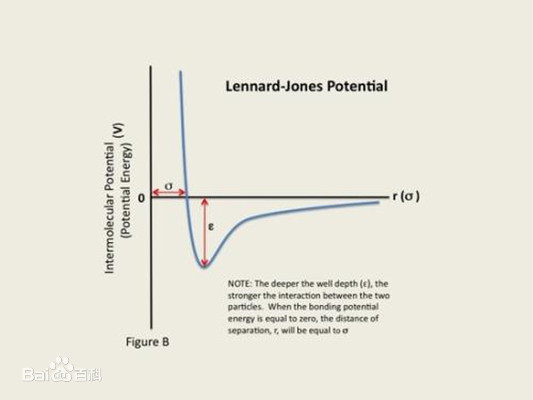
\includegraphics[width=0.45\textwidth]{LJpotential}}  
		实际的相互作用势V(x) 较L-J势更复杂,试求其在平衡位置附近的二阶近似	
	\end{exampleblock}
\end{frame}

\begin{frame}
	\frametitle{}
	\alert{解:} 	不管多复杂,在平衡位置 ($x=a$)附近可泰勒展开
	\begin{equation*}
		V(x)=V(a) +\frac{1}{1!} \frac{\partial V}{\partial x} |_{x=a} (x-a) +\frac{1}{2!} \frac{\partial ^2 V}{\partial x ^2} |_{x=a} (x-a) ^2 + ... 
	\end{equation*}
	一阶导应为零,二阶近似可写为 \\
	$\displaystyle  \begin{array}{lllllllll}
		V(x) &\approx V(a)+\dfrac{1}{2!} \dfrac{\partial ^2 V}{\partial x ^2} |_{x=a} (x-a) ^2   \\
		& =V_0+\dfrac{1}{2} k (x-a) ^2 
	\end{array}$\\
	取坐标原点为($a, V_0 $), 得:\\
	\begin{equation*}
		V(x)=\dfrac{1}{2} k x^2 
	\end{equation*}	
\end{frame}

\begin{frame}
	\frametitle{}
	\begin{block}{弹性势}
		~~\\
		弹簧力正是势函数V(x) 在平衡位置附近的二阶近似\\
		\begin{equation*}
			F=-\frac{ \partial V}{\partial x}=-kx 
		\end{equation*}	
		 把势函数V(x) 改写成弹性势能:\\
		\begin{equation*}
			U(x)=\dfrac{1}{2} \mu \omega ^2 x^2 
		\end{equation*}
	\end{block}	
\end{frame}	

\subsection{量子谐振子方程}

\begin{frame}
	\frametitle{量子谐振子方程}
	\begin{exampleblock} {例2、求解谐振子薛定谔方程}
	\begin{equation*}
		i\hbar \frac{\partial }{\partial t} \Psi (x,t ) =[ -\frac{\hbar^2}{2\mu } \frac{d ^2}{x^2} + \frac{1}{2} \mu \omega ^2 x^2   ] \Psi (x, t ) 
	\end{equation*}
	\end{exampleblock}
	\alert{解:} 	令$\Psi (x,t) =\Psi(x) T(t) $ ,  代回方程\\
	时间和位置分离变量:\\
	时间函数: $T(t)  = \exp(-i E t /\hbar) $ \\
	位置函数满足定态薛定谔方程\\
	\begin{equation*}
		\left [ -\frac{\hbar^2}{2\mu} \frac{\mathrm{d} ^2}{\mathrm{d} x^2} +\frac{1}{2}\mu \omega^2 x^2  \right ]\Psi(x)=E\Psi(x) 
	\end{equation*}	
\end{frame}

\begin{frame}
	\frametitle{}
	整理:\\
	\begin{equation*}
		\frac{1}{\dfrac{\mu\omega}{\hbar}} \frac{\mathrm{d} ^2\Psi}{\mathrm{d} x^2} +	\left ( \frac{2E}{\omega \hbar} -\frac{\mu \omega}{\hbar} x^2 \right )\Psi=0
	\end{equation*}
	令:~~$ \xi =\alpha x$,做自变量伸缩变换 \\
	\begin{equation*}
		\frac{\mathrm{d} \Psi}{\mathrm{d} x} =\frac{\mathrm{d} \Psi}{\mathrm{d} \xi} \frac{\mathrm{d} \xi}{\mathrm{d} x}  = \alpha \frac{\mathrm{d} \Psi}{\mathrm{d} \xi}
	\end{equation*}
	\begin{equation*}
		\frac{\mathrm{d} \Psi ^2 }{\mathrm{d} x ^2} =\frac{\mathrm{d}}{\mathrm{d} x}  ( \alpha \frac{\mathrm{d} \Psi}{\mathrm{d} \xi} ) = \alpha ^2 \frac{\mathrm{d} ^2 \Psi}{\mathrm{d} \xi ^2} 
	\end{equation*}
	代回方程, 得\\
	\begin{equation*}
		\left[ \frac{\hbar ^2 \alpha ^2 }{2\mu} \frac{\mathrm{d}}{\mathrm{d} \xi ^2}  + (E- \frac{\mu \omega ^2 \xi ^2}{2 \alpha ^2}  ) \right] \Psi(\xi) =0
	\end{equation*}	
\end{frame}

\begin{frame}
	\frametitle{}
	同除二阶导数项系数, 得\\
	\begin{equation*}
		\left[ \frac{\mathrm{d}}{\mathrm{d} \xi ^2}  + \frac{2\mu}{\hbar ^2 \alpha ^2 } (E- \frac{\mu \omega ^2 \xi ^2}{2 \alpha ^2}  ) \right] \Psi(\xi) =0
	\end{equation*}
	令 $\dfrac{\mu ^2 \omega ^2 }{\hbar ^2 \alpha ^ 4}=1 $,得伸缩系数:\\
	\begin{equation*}
		\alpha ^2= \frac{\mu\omega}{\hbar}
	\end{equation*}
	引入特征值\\
	\begin{equation*}
		\lambda = \frac{2E}{\omega \hbar}
	\end{equation*}
	得二阶常微分方程\\
	\begin{equation*}
		\left[ \frac{\mathrm{d} ^2\Psi}{\mathrm{d} \xi^2} + \left( \lambda - \xi^2 \right) \right] \Psi=0
	\end{equation*}
\end{frame}

\begin{frame}
	\frametitle{}
	考虑渐近行为, 当 $ |x| \to \infty,  \xi \to \infty$,有 $ \xi ^2  \gg  \lambda $,方程可近似为 \\
	\begin{equation*}
		\left(\frac{\mathrm{d} ^2}{\mathrm{d} \xi^2} - \xi^2 \right) \Psi=0
	\end{equation*}
	方程并无表达式解,但通过检验平方指数函数的导数\\
	\begin{equation*}
		\frac{d^2 }{d \xi ^2} \exp(\frac{\xi ^2}{2}) =(\xi ^2 +1)  \exp(\frac{\xi ^2}{2}) 
	\end{equation*}    
	\begin{equation*}
		\frac{d^2 }{d \xi ^2} \exp( - \frac{\xi ^2}{2}) =(\xi ^2 -1)  \exp( - \frac{\xi ^2}{2}) 
	\end{equation*}     	
\end{frame}

\begin{frame}
	\frametitle{}
	当 $ \xi \to \infty$, 这两导数可近似为:\\
	\begin{equation*}
		(\xi ^2 )  \exp( \frac{\xi ^2}{2}) ~~, ~~ (\xi ^2 )  \exp( - \frac{\xi ^2}{2}) 
	\end{equation*}     
	因此,极限状态解应与如下函数相关联
	\begin{equation*}
		C_1  \exp( \frac{\xi ^2}{2}) + C_2   \exp( - \frac{\xi ^2}{2})  
	\end{equation*}     
	考虑到波函数的有界性,应删除发散项(第一项),得极限状态波函数的简洁形式
	\begin{equation*}
		\Psi_\infty (\xi)  \sim C_2 \exp( - \frac{\xi ^2}{2})  
	\end{equation*}   
\end{frame}

\begin{frame}
	\frametitle{}
	现考虑非极限状态,解函数可写成: 
	\begin{equation*}
		\Psi(\xi) = H(\xi) e^{-\xi^2/2 }  
	\end{equation*}   
	解函数的确定等价于多项式函数 H 的确定。\\
	对上式求导:\\
	\begin{equation*}
		\Psi'(\xi) = H'(\xi) e^{-\xi^2/2 } -  H(\xi) \xi e^{-\xi^2/2 } 
	\end{equation*}  
	\begin{equation*}
		\Psi''(\xi) = \left[  \left( \xi^2 -1 \right) H -2\xi H' +H''  \right] e^{-\xi^2/2}
	\end{equation*}  
	代回原方程  $ \displaystyle \dfrac{\mathrm{d} ^2\Psi}{\mathrm{d} \xi^2} + \left( \lambda - \xi^2 \right) \Psi=0 $  \\ 
\end{frame}

\begin{frame}
	\frametitle{}
	得关于多项式$H(\xi)$的方程: \\  
	\begin{equation*}
		H'' -2 \xi H' +(\lambda -1) H=0 
	\end{equation*}  
	取$\lambda -1= 2n $,方程转化为n阶厄密方程
	\begin{equation*}
		H'' -2 \xi H' +2n H=0 
	\end{equation*}  
	由
	\begin{equation*}
		\lambda = 2n +1 = \frac{2E}{\hbar  \omega}  
	\end{equation*}  
	解出能量固有值(能级)
	\begin{equation*}
		E_n=\left(n+\frac{1}{2}\right) \hbar \omega, ~~~  ( n=0,1,2, ...)  
	\end{equation*}  
	固有函数由n阶厄密方程给出......
\end{frame}

%%%%%%%%%%%%%%%%%%%%%%%%%%%%%%%%%%
\subsection{厄密方程}

\begin{frame}
	\frametitle{厄密方程}
	\begin{exampleblock} {例3、求解n阶厄密方程}
		\begin{equation*}
			H'' -2 \xi H' +2n H=0 
		\end{equation*}  
	\end{exampleblock}
	\alert{解:} 	幂级数方法求解,令:
	\begin{equation*}
		H=\sum_{k=0}^{\infty} c_k \xi ^k
	\end{equation*}     
	求一阶导和二阶导,代回厄密方程,可得系数递推式:
	\begin{equation*}
		c_{k+2} = \frac{ 2(k-n)}{(k+2)(k+1) } c_k, ~~  \left( k=0,1,2,3, ...  \right)
	\end{equation*}   
\end{frame}

\begin{frame}
	\frametitle{}
	分偶数阶和奇数阶写
	\begin{equation*}
		c_{2m} = (-1) ^m \frac{2^mn(n-2)(n-4) ... (n-2m+2)  } {(2m)!} c_0
	\end{equation*}   
	显然有 $ c_{2m} =0~, ~~(2m>n)$
	\begin{equation*}
		c_{k} = (-1) ^m \frac{2^mn !! } {k!} c_0, ~~~(2m=k)
	\end{equation*}   
	\begin{equation*}
		c_{2m+1} = (-1) ^m \frac{2^m (n-1) (n-3)(n-5)...(n-2m+1)  } {(2m+1)!} c_1
	\end{equation*}   
	显然有 $ c_{2m+1} =0~, ~~(2m+1>n)$
	\begin{equation*}
		c_{k} = (-1) ^m \frac{2^m n!! }{k!} c_1, ~~~ (2m+1=k)
	\end{equation*}  
\end{frame}

\begin{frame}
	\frametitle{}
	所有系数求得,幂级数得解\\
	$\displaystyle \begin{cases}
		y_1(\xi)  = [1- \dfrac{2n}{2!} \xi^2+ \dfrac{2^2n(n-2)}{4!} \xi^4 -...  ] \\
		\\
		y_2(\xi)  = [\xi- \dfrac{2(n-1)}{3!} \xi^3+ \dfrac{2^2(n-1)(n-3) }{5!}\xi^5 -...  ]
	\end{cases}$ \\
	n阶厄密方程的解:
	\begin{equation*}
		H(\xi) =c_0y_1(\xi)+c_1 y_2(\xi).
	\end{equation*}   
 	 量子谐振子方程的解:
	\begin{equation*}
		\Psi(\xi) = [c_0y_1(\xi)+c_1 y_2(\xi) ]e^{-\xi^2/2 }  
  	\end{equation*}   
  	根据波函数的有界性性质, H应取多项式 (不能为无穷级数)。当n为偶数时 , $c_1=0$ , 当n为奇数时 , $c_0=0$ 。 待定系数由定解条件给出...
\end{frame}

\begin{frame}
	\frametitle{}
		为了更好地描述,将系数递推式降幂排列,现令最高次项系数为:
	\begin{equation*}
		c_n =2^n
	\end{equation*}  
	系数递推式可写为:
	\begin{equation*}
		c_{k-2} = -\frac{k(k-1) } { 2(n-k+2)}  c_k
	\end{equation*} 
	\begin{equation*}
		c_{n-2} = -\frac{n(n-1) } { 2\times2}  c_n
	\end{equation*} 
	\begin{equation*}
		c_{n-4} = (-1)^2 \frac{n(n-1)(n-2) (n-3) } { 2\times2\times 4}  2^n
	\end{equation*} 
		\begin{equation*}
		c_{n-2m} = (-1)^m \frac{n! } { 2^m (2m) !! (n-2m)!}  2^n =(-1)^m \frac{n! } {  m ! (n-2m)!}  2^{n-2m} 
	\end{equation*} 
\end{frame}

\begin{frame}
	\frametitle{}
	厄密方程的解为厄米多项式:
	\begin{equation*}
		H_n(\xi) =\sum_{m=0}^{M}  (-1)^m \frac{n! } {  m ! (n-2m)!}  2^{n-2m} \xi^{n-2m} ,  ~~~ M=[n/2]
	\end{equation*}   
	量子谐振子的解为
	\begin{equation*}
		\Psi_n(\xi) = N_n \exp(-\frac{\xi ^2}{2}) H_n(\xi) 
	\end{equation*}   
	归一化解:(...)
	\begin{equation*}
		\Psi_n(x) = \left( \frac{\alpha}{\sqrt{\pi} 2^n n!}  \right) ^{1/2}  \exp(-\frac{ \alpha^2 x^2}{2}) H_n( \alpha x) 
	\end{equation*}  
	定态波函数为
	\begin{equation*}
		\Psi_n(x,t) = \left( \frac{\alpha}{\sqrt{\pi} 2^n n!}  \right) ^{1/2}  \exp(-\frac{ \alpha^2 x^2}{2} -\frac{i}{\hbar} E_n t ) H_n( \alpha x) 
	\end{equation*}  	
\end{frame}

\begin{frame}
	\frametitle{作业:}
	1、计算积分\\ 
	$\begin{array}{lllllllll}
		 &\int\limits_{0}^{+\infty} e^{-x^2 /2} dx
	\end{array}$ \\ \vspace{0.6em}
	2、 根据厄米多项式表达式,写出前五个厄米多项式,并分析$H'_n (x)$ 与$H_{n-1} (x)$  之间的联系\\ \vspace{0.6em}
	3、 求解厄米方程\\ \vspace{0.6em}
	$\begin{array}{lllllllll}
		& \dfrac{d^2 H}{d x^2} -2x \dfrac{d y}{d x} +4n H =0 		
	\end{array}$ \\ \vspace{0.6em}
	4、  列出厄米方程的几种形式,说明厄米方程的特点
\end{frame}

%%%%%%%%%%%%%%%%%%%%%%%%%%%%%%%%%%%%%%%%%%%%%
\section{4.厄密多项式及性质}

\subsection{生成函数}

\begin{frame}
	\frametitle{ 生成函数 }
	\begin{exampleblock} { 例1、求厄密多项式的生成函数 }
		找一个函数,它的展开系数刚好就是Hermite 多项式
		 \begin{equation*}
			w(x,t)=e^{2xt-t^2}
		\end{equation*}
		试证明,上述二元函数就是Hermite多项式的一个母函数
	\end{exampleblock}
	\alert {解:}	把函数做关于变量t的Taylor 展开:
	\begin{equation*}
		w(x,t) =\sum_{n=0}^{\infty} \frac{1}{n!}  c_n(x) t^n
	\end{equation*}
	需证明:
	\begin{equation*}
		\left[  \frac{d^2}{dx^2} -2x\frac{d}{dx} +2n  \right] c_n(x)=0
	\end{equation*}
\end{frame}

\begin{frame}
	\frametitle{  }
	\textbf{证明:}	1)、由 $  \dfrac{\partial w}{\partial x} =2t e^{2xt-t^2} =2t ~w(x,t) $, 得 \\ 
	$ \sum\limits_{n=0}^{\infty} \dfrac{1}{n!}  c~'_n(x) t^n  = 2t  \sum\limits_{n=0}^{\infty} \dfrac{1}{n!}  c_n(x) t^n $ \\
	\hspace{2.3cm}	$=  \sum\limits_{n=0}^{\infty} \dfrac{1}{n!}  2c_{n}(x) t^{n+1} $\\
	\hspace{2.3cm}	$=  \sum\limits_{n=1}^{\infty} \dfrac{1}{n!}  2nc_{n-1}(x) t^{n}   $ \\
	比较系数,有:\\
	\hspace{2.1cm}	{ $c~'_n(x)=2nc_{n-1}(x)$} \\  \vspace{0.3cm}
	\hspace{2.1cm}	$c~''_n(x)=2nc~'_{n-1}(x)=4n(n-1)c_{n-2}(x)$ \\  	
\end{frame}

\begin{frame}
	\frametitle{  }
	2)由 $  \dfrac{\partial w}{\partial t} =2(x-t) e^{2xt-t^2} =2(x-t) ~w(x,t) $, 得 \\ 
	\hspace{2.1cm}		$  \dfrac{\partial w}{\partial t} +2(t-x) ~w(x,t) =0$ \\ 
	把展开式代入上式\\ 
	{$  \sum\limits_{n=1}^{\infty} \dfrac{1}{n!}n c_n(x) t^{n-1} +\sum\limits_{n=0}^{\infty} \dfrac{1}{n!}2(t-x) c_n(x)t^n=0$ } \\ \vspace{0.3cm}
	{$ \sum\limits_{n=1}^{\infty} \dfrac{1}{n!}n c_n(x) t^{n-1} +\sum\limits_{n=0}^{\infty} \dfrac{-2x}{n!} c_n(x)t^n +\sum\limits_{n=0}^{\infty}\dfrac{2}{n!} c_n(x)t^{n+1}=0$ } \\ \vspace{0.3cm}
	{$ \sum\limits_{n=0}^{\infty} \dfrac{1}{n!} c_{n+1}(x) t^{n} +\sum\limits_{n=0}^{\infty} \dfrac{-2x}{n!} c_n(x)t^n +\sum\limits_{n=1}^{\infty}\dfrac{2n}{n!} c_{n-1}(x)t^n=0$ } 
\end{frame}

\begin{frame}
	\frametitle{  }
	比较系数,有:\\
	\hspace{2.1cm}	{  $ c_{n+1}(x) -2xc_n(x) +2nc_{n-1} (x) =0 $} \\ \vspace{0.3cm}
	\hspace{2.1cm}	{  $ c_{n}(x) -2xc_{n-1}(x) +2(n-1)c_{n-2} (x) =0 $} \\ 
	3) 把(1)中得到的结论 \\
	\hspace{2.1cm}	{ $c~'_n(x)=2nc_{n-1}(x)$} \\  \vspace{0.3cm}
	\hspace{2.1cm}	$c~''_n(x)=4n(n-1)c_{n-2}(x)$ \\  
	代入(2)中得到的结论,得:\\
	\hspace{2.1cm} $  c_{n}(x) - \dfrac{x}{n}c~'_{n}(x) +\dfrac{1}{2n}c~''_{n} (x) =0 $ \\
	整理为:
	\begin{equation*}
 	    \left[  \dfrac{d^2}{dx^2} -2x\frac{d}{dx} +2n  \right] c_n(x)=0 
	\end{equation*}
 	\textcolor{red}{证毕!}\\
	即有: $c_n(x)=H_n(x)  $ 
\end{frame}

\subsection{性质}
\begin{frame}
	\frametitle{递推公式 }
	{  既然: $c_n(x)=H_n(x) $}  \\ \vspace{0.3cm}
	\hspace{1cm} 	{  $c~'_n(x)=2nc_{n-1}(x)    $ }   \\ 
	{  $ ~\to~~  H~'_n(x)=2nH_{n-1}(x)    $}   \\ \vspace{0.3cm}
	\hspace{1cm} 	{  $ c_{n}(x) -2xc_{n-1}(x) +2(n-1)c_{n-2} (x) =0  $ }   \\ 
	{  $~\to~~   H_{n}(x) -2xH_{n-1}(x) +2(n-1)H_{n-2} (x) =0  $ } \\ \vspace{0.3cm}
	有: $H_0(x)=1,  H_1(x)=2x, $	
\end{frame}

\begin{frame}
	\frametitle{ 微分形式 }
	$ \displaystyle w(x,t) =\sum_{n=0}^{\infty} \frac{1}{n!}  c_n(x) t^n $, ~~~~
	{ $ \displaystyle w(x,t) =\sum_{n=0}^{\infty} \frac{1}{n!}  H_n(x) t^n  $} \\
	由Taylor展式,知:\\
	{ $ \displaystyle  H_n(x) = \left[  \frac{\partial ~^n w  }{\partial t^n}  \right] _{t=0} $}\\ 
	\hspace{1cm} {$ 	\displaystyle  =e^{x^2}   \left[  \frac{\partial ^n }{\partial t^n}  e^{-(x-t)^2}   \right] _{t=0}   $}  \\ 
	\hspace{1cm} {$ 	\displaystyle  =(-1) ^n e^{x^2}   \left[  \frac{d~^n }{d~u^n}  e^{-u^2}   \right] _{u=x}   $}  \\ 
	{$ 	\displaystyle H_n(x) =(-1) ^n e^{x^2}  \frac{d~^n }{d~x^n}  e^{-x^2}   $}  \\ 
\end{frame}

\begin{frame}
	\frametitle{ 正交性 }
	\begin{exampleblock} { 例2、证明厄密多项式正交性 }
	是带权函数($\rho(x) =exp(-x^2)$)的正交函数系:\\
	{$ \displaystyle  
	\left\{  
	\begin{array}{ccccc}
		\int\limits_{-\infty}^{+\infty} e^{-\xi^{2}} H_m(\xi) H_n(\xi)d\xi &=&0 ~~~~~~\\
		\int\limits_{-\infty}^{+\infty} e^{-\xi^{2}} H_n(\xi) H_n(\xi)d\xi &=&2^n n! \sqrt{\pi}  
	\end{array}
	\right.  
	$} 
	\end{exampleblock}
\alert {证明:}	
	谐振子方程:{ $ \displaystyle \dfrac{\mathrm{d} ^2\Psi}{\mathrm{d} \xi^2} + \left( \lambda - \xi^2 \right) \Psi=0  $  }  \\
	代入$\lambda=2n+1 $~\\
	$\to   \Psi''_n +(2n+1-\xi^2) \Psi_n =0$ \\
	解为: $u_n(x)=H_n(\xi) e^{-\xi^{2}/2}$ , 代回方程,得:
\end{frame}

\begin{frame}
	\frametitle{  }
	$u''_n+ (2n+1-\xi^2) u_n =0    ~, ~u''_m+ (2m+1-\xi^2) u_m =0  $\\  \vspace{0.3cm}
	$u_mu''_n +(2n+1-\xi^2) u_mu_n =0 $\\ 
	$u_nu''_m+ (2n+1-\xi^2) u_nu_m =0  $  \\  \vspace{0.3cm}
	$u_mu''_n -u_nu''_m +2(n-m)u_nu_m=0 $\\  \vspace{0.3cm}
	$ \int\limits_{-\infty}^{+\infty} [u_mu''_n -u_nu''_m] d\xi  $\\
	\hspace{2cm} 	$= [u_mu''_n -u_nu''_m] \left |_{-\infty} ^{+\infty}  \right. -\int\limits_{-\infty}^{+\infty} [u'_mu'_n -u'_nu'_m] d\xi =0$\\   
	因此	$ 2(n-m) \int\limits_{-\infty}^{+\infty} u_nu_m d\xi =0$ \\   \vspace{0.3cm}
	即:{ $ \int\limits_{-\infty}^{+\infty} e^{-\xi^{2}} H_m(\xi) H_n(\xi)d\xi =0 $ }	
\end{frame}

\begin{frame}
	\frametitle{  }
	由递推公式:\\
	{$H_{n} -2xH_{n-1} +2(n-1)H_{n-2} =0  $ } \\
	=> 	{ $H^2_{n}-2xH_n H_{n-1}+2(n-1) H_n H_{n-2} =0  $ }\\   \vspace{0.3cm}
	{$H_{n+1} -2xH_{n} +2nH_{n-1} =0  $ } \\
	=>   { $H_{n+1} H_{n-1}-2xH_{n} H_{n-1}+2nH^2_{n-1} =0  $ } \\  \vspace{0.3cm}
	两次相减\\
     $H^2 _n(\xi) -H_{n+1} H_{n-1}=2n H^2 _{n-1}(\xi) - 2(n-1) H_n H_{n-2}$ \\	  \vspace{0.3cm}
	乘以权重函数再积分,  得积分递推式:\\
	{$\int\limits_{-\infty}^{+\infty} e^{-\xi^2} H^2 _n(\xi) d\xi =2n \int\limits_{-\infty}^{+\infty} e^{-\xi^{2}} H^2 _{n-1}(\xi) d\xi$ }\\	
\end{frame}	

\begin{frame}
	\frametitle{  }
	{$\int\limits_{-\infty}^{+\infty} e^{-\xi^2} H^2 _n(\xi) d\xi =2n \int\limits_{-\infty}^{+\infty} e^{-\xi^{2}} H^2 _{n-1}(\xi) d\xi$ }\\
	$= 2n \times 2(n-1) \int\limits_{-\infty}^{+\infty} e^{-\xi^{2}} H^2 _{n-2}(\xi) d\xi$  \\
	$= 2n \times 2(n-1) ... (2(n-n)) \int\limits_{-\infty}^{+\infty} e^{-\xi^{2}} H^2 _{0}(\xi) d\xi$  \\
	$= 2^n n! \int\limits_{-\infty}^{+\infty} e^{-\xi^{2}} H^2 _{0}(\xi) d\xi$  \\	
	$= 2^n n! \int\limits_{-\infty}^{+\infty} e^{-\xi^{2}} d\xi$  \\	
	$= 2^n n! \sqrt{\pi} $ \\	
\end{frame}	

\subsection{归一化系数}

\begin{frame}
	\frametitle{求归一化系数}
	固有解为
	\begin{equation*}
		\Psi_n(\xi) = N_n \exp(-\frac{\xi ^2}{2}) H(\xi) 
	\end{equation*}   
	\begin{equation*}
		\int\limits_{-\infty}^{+\infty} [N_n \exp(-\frac{\xi ^2}{2}) H(\xi) ]^2d\xi  =N^2 _n 2^n n! \sqrt{\pi}=1
	\end{equation*}  
	\begin{equation*}
    	N_n=\dfrac{1}{(2^n n! \sqrt{\pi}) ^{1/2}}
	\end{equation*}    
\end{frame}	

\begin{frame}
	\frametitle{  }
	归一化固有函数:\\  
	{ $  \displaystyle  \Psi_n(x) =  \left(  \dfrac{\alpha}{\sqrt{\pi} 2^n n! } \right) ^{1/2} e^{-a^2 x^2}  H_n(\alpha x)  $ } \\ 
	定态波函数: \\
	{ $  \displaystyle  \Psi_n(x,t) =  \Psi_n(x) e^{-\dfrac{i}{\hbar} E_n t } $} \\
	{$  \displaystyle = \left(  \dfrac{\alpha }{\sqrt{\pi} 2^n n! } \right) ^{1/2} e^{-a^2 x^2 -\dfrac{i}{\hbar} E_n t }  H_n(\alpha  x)  $ } \\  
	叠加解:\\
	{\large $  \displaystyle \Psi(x,t) =\sum a_n \Psi_n(x,t)  $} \\	
\end{frame}	

\begin{frame}
	\frametitle{  }
	下图给出了基态和第一激发态函数及概率分布\\
	%\usetikzlibrary {datavisualization.formats.functions} 
	\begin{tikzpicture}[baseline, scale=.7]
	\datavisualization [ scientific axes, 
		visualize as smooth line/.list={sin,cos}, style sheet=strong colors,
		style sheet=vary dashing,
		sin={label in legend={text=$\Psi_0(x)$}}, 
		cos={label in legend={text=$\Psi_1(x) $}}, 
		data/format=function ]
		data [set=sin] {
			var x : interval [-3:3];
			func y = 1/sqrt(sqrt(pi))* exp(-0.5 * \value x * \value x  )  ;
		}
		data [set=cos] {
			var x : interval [-3:3];
			func y = 2*\value x /sqrt(2*sqrt(pi))* exp(-0.5 * \value x * \value x  )  ;
		};
	\end{tikzpicture}	
   %\usetikzlibrary {datavisualization.formats.functions} 
   	\begin{tikzpicture}[baseline, scale=.7]
   	\datavisualization [ scientific axes, 
   		visualize as smooth line/.list={sin,cos}, style sheet=strong colors,
   		style sheet=vary dashing,
   		sin={label in legend={text=$|\Psi_0(x)|^2$}}, 
   		cos={label in legend={text=$|\Psi_1(x)|^2$}}, 
   		data/format=function ]
   		data [set=sin] {
   			var x : interval [-3:3];
   			func y = 1/sqrt(pi)* exp(- \value x * \value x  )  ;
   		}
   		data [set=cos] {
   		var x : interval [-3:3];
   		func y = 2*\value x * \value x /sqrt(pi)* exp(- \value x * \value x  )  ;
   		};
   \end{tikzpicture}
\end{frame}	

\begin{frame}
	\frametitle{ 课堂测试! }	
	\begin{exampleblock} {课堂测试题1:}
		求处于如下势场:
		\begin{equation*}
			V(x)= \frac{1}{2} \mu \omega ^2 x^2  +\mu
		\end{equation*}
		中粒子的能量固有值和定态波函数。
	\end{exampleblock}	
\end{frame}	

\begin{frame}
	\frametitle{ 作业 }
	1、将函数$f(x)=x^3+2x^2 +1$ 按厄米多项式展开\\ 
	参考答案:$f(x) =\dfrac{1}{8} H_3 + \dfrac{1}{2} H_2 +\dfrac{3}{4} H_1 + 2 H_0 $\\
	2、写出厄米多项式的递推公式,并求 $H_n(0) ,   H'_n(0) , H_n(1) ,   H'_n(1)  $\\ 
	3、求解如下初值问题\\
	\begin{equation*}
		\left\{ 
		\begin{aligned}
			& i \hbar \dfrac{\partial \Psi}{\partial t}  = \left[  -\dfrac{\hbar ^2}{2\mu} \dfrac{\partial ^2}{\partial x^2} +\dfrac{1}{2}  \mu \omega ^2 x ^2 \right] \Psi \\
			& \Psi(x, 0) =\psi(x)
		\end{aligned} 
		\right.
	\end{equation*}
\end{frame}	

\begin{frame}
	\frametitle{ 作业 }
	4、	电荷为q的谐振子,受到沿 x 方向的外电场$\xi $的作用时,其势场为:
	\begin{equation*}
		V(x)= \frac{1}{2} \mu \omega ^2 x^2  +q\xi x  
	\end{equation*}
	求解其能量固有值和定态波函数。(移轴法)
\end{frame}

\begin{frame}
	\frametitle{课外读物和思考}
	薛定谔方程的数值解法:\\
	Matlab or Python or VASP
\end{frame}	
%%%%%%%%%%%%%%%%%%%%%%%%%%%%%%%%%%%%%%%%%%%%%%